% Kompilieren mit: TEXINPUTS=minted/source: pdflatex -shell-escape %
\documentclass[12pt,compress,ngerman,utf8,t]{beamer}
\usepackage[ngerman]{babel}
\usepackage{ragged2e}
\usepackage{comment}
\usepackage{minted}
\usepackage{wasysym}
\usepackage{tikz}
\usetikzlibrary{calc}
\usepackage[all]{xy}
\usepackage[protrusion=true,expansion=false]{microtype}

\DeclareSymbolFont{extraup}{U}{zavm}{m}{n}
\DeclareMathSymbol{\varheart}{\mathalpha}{extraup}{86}
\DeclareMathSymbol{\vardiamond}{\mathalpha}{extraup}{87}

\DeclareUnicodeCharacter{2237}{$\dblcolon$}
\DeclareUnicodeCharacter{21D2}{$\Rightarrow$}
\DeclareUnicodeCharacter{2192}{$\rightarrow$}

\title[Initiale Algebren]{\smiley{} Initiale Algebren \smiley}
\author[Augsburger Curry Club]{}
\date[2016-06-16]{}

\usetheme{Warsaw}

\useinnertheme{rectangles}

\usecolortheme{seahorse}
\definecolor{mypurple}{RGB}{150,0,255}
\setbeamercolor{structure}{fg=mypurple}
\definecolor{myred}{RGB}{150,0,0}
\setbeamercolor*{title}{bg=myred,fg=white}
\setbeamercolor*{titlelike}{bg=myred,fg=white}

\usefonttheme{serif}
\usepackage[T1]{fontenc}
\usepackage{libertine}

\newcommand{\slogan}[1]{%
  \begin{center}%
    \setlength{\fboxrule}{2pt}%
    \setlength{\fboxsep}{8pt}%
    {\usebeamercolor[fg]{item}\fbox{\usebeamercolor[fg]{normal text}\parbox{0.91\textwidth}{#1}}}%
  \end{center}%
}

\definecolor{darkred}{RGB}{220,0,0}
\newcommand{\hcancel}[5]{%
    \tikz[baseline=(tocancel.base)]{
        \node[inner sep=0pt,outer sep=0pt] (tocancel) {#1};
        \draw[darkred, line width=1mm] ($(tocancel.south west)+(#2,#3)$) -- ($(tocancel.north east)+(#4,#5)$);
    }%
}%

\renewcommand{\C}{\mathcal{C}}
\newcommand{\D}{\mathcal{D}}
\newcommand{\id}{\mathrm{id}}
\newcommand{\Id}{\mathrm{Id}}
\newcommand{\Hask}{\mathrm{Hask}}

\setbeamertemplate{navigation symbols}{}
\setbeamertemplate{headline}{}

\setbeamertemplate{title page}[default][colsep=-1bp,rounded=false,shadow=false]
\setbeamertemplate{frametitle}[default][colsep=-2bp,rounded=false,shadow=false,center]

\newcommand*\oldmacro{}%
\let\oldmacro\insertshorttitle%
\renewcommand*\insertshorttitle{%
  \oldmacro\hfill\insertframenumber\,/\,\inserttotalframenumber\hfill}

\newcommand{\hil}[1]{{\usebeamercolor[fg]{item}{\textbf{#1}}}}
\setbeamertemplate{frametitle}{%
  \vskip1em%
  \leavevmode%
  \begin{beamercolorbox}[dp=1ex,center]{}%
      \usebeamercolor[fg]{item}{\textbf{\textsf{\Large \insertframetitle}}}
  \end{beamercolorbox}%
}

\setbeamertemplate{footline}{%
  \leavevmode%
  \hfill%
  \begin{beamercolorbox}[ht=2.25ex,dp=1ex,right]{}%
    \usebeamerfont{date in head/foot}
    \insertframenumber\,/\,\inserttotalframenumber\hspace*{1ex}
  \end{beamercolorbox}%
  \vskip0pt%
}

\newcommand{\backupstart}{
  \newcounter{framenumberpreappendix}
  \setcounter{framenumberpreappendix}{\value{framenumber}}
}
\newcommand{\backupend}{
  \addtocounter{framenumberpreappendix}{-\value{framenumber}}
  \addtocounter{framenumber}{\value{framenumberpreappendix}}
}

\setbeameroption{show notes}
\setbeamertemplate{note page}[plain]

\begin{document}

% http://www.goodwp.com/images/201311/goodwp.com_30317.jpg
{\usebackgroundtemplate{
\includegraphics[height=\paperheight]{images/forest}}
\frame{\titlepage\vspace*{16em}}}

\frame{\tableofcontents}

\section{Motivation}

\begin{frame}\frametitle{Motivation}
  In der Mathematik und theoretischen Informatik untersucht man oft
  \hil{Fixpunktgleichungen}:
  \[ x = f(x) \]
  Oft ist man am \hil{kleinsten} oder \hil{größten} Fixpunkt interessiert:
  \[ \mu f \qquad\text{oder}\qquad \nu f \]

  \centering
  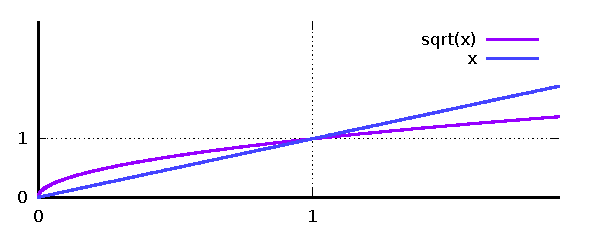
\includegraphics{fixpunkt}
  \par
\end{frame}

\begin{frame}[fragile]\frametitle{Motivation}
  In der theoretischen Informatik benötigt man aber auch
  eine höhere Art von Fixpunkt"`gleichungen"':
  \[ X \cong F(X) \]

  \hil{Initiale Algebren} verallgemeinern kleinste Fixpunkte,
  \hil{terminale Koalgebren} verallgemeinern größte Fixpunkte.
  \medskip

  Wir klären heute folgende Frage: Was bedeutet
  \begin{minted}{haskell}
     data Nat = Zero | Succ Nat
  \end{minted}
  eigentlich wirklich?
  \medskip

  Zunächst:
  "`keine Bottoms, alles endlich"'.
\end{frame}


\section{Algebren}

\subsection{Definition}

\begin{frame}[fragile]\frametitle{Algebren}
  Eine \hil{Algebra} für einen Funktor $F : \C \to \C$ besteht aus
  \begin{itemize}
    \item einem Objekt $A \in \C$ und
    \item einem Morphismus $\alpha : F(A) \to A$ in~$\C$.
  \end{itemize}

  \begin{minted}{haskell}
-- Beispielfunktor
data F a = Nil | Cons Int a

instance Functor F where
    fmap f Nil        = Nil
    fmap f (Cons x r) = Cons x (f r)

-- Beispielalgebra
productA :: F Int -> Int
productA Nil        = 1
productA (Cons x r) = x * r
  \end{minted}
\end{frame}

\begin{frame}[fragile]{Algebren sind nicht rar!}
  \begin{minted}{haskell}
data F a = Nil | Cons Int a

productA :: F Int -> Int
productA Nil        = 1
productA (Cons x r) = x * r

lengthA :: F Int -> Int
lengthA Nil        = 0    
lengthA (Cons _ r) = 1 + r

allNonzeroA :: F Bool -> Bool
allNonzeroA Nil        = True
allNonzeroA (Cons x r) = x /= 0 && r
  \end{minted}
\end{frame}

\begin{frame}[fragile]{Ein besonderes Beispiel}
  \begin{minted}{haskell}
data F a = Nil | Cons Int a

prodA :: F Int -> Int
prodA Nil        = 1
prodA (Cons x r) = x * r

allNonzeroA :: F Bool -> Bool
allNonzeroA Nil        = True
allNonzeroA (Cons x r) = x /= 0 && r

initialA :: F [Int] -> [Int]
initialA Nil        = []
initialA (Cons x r) = x : r
  \end{minted}
\end{frame}


\subsection{Morphismen zwischen Algebren}

\begin{frame}[fragile]{Morphismen zwischen Algebren}
  Ein \hil{Morphismus} zwischen~$F$-Algebren
  $\alpha : F(A) \to A$ und $\beta : F(B) \to B$ ist ein Morphismus
  $g : A \to B$
  sodass das folgende Diagramm kommutiert.
  \[ \xymatrix{
    F(A) \ar[r]^\alpha\ar[d]_{\operatorname{fmap} g} & A \ar[d]^g \\
    F(B) \ar[r]_\beta & B
  } \]

  \begin{minted}{haskell}
data F a = Nil | Cons Int a

g :: Int -> Bool
g x = x /= 0
-- g . prodA = allNonzeroA . fmap g
  \end{minted}
\end{frame}


\subsection{Initiale Algebren}

\begin{frame}[fragile]{Initiale Algebren}
  Die "`besondere Beispielalgebra"' hat eine \hil{universelle Eigenschaft}:
  Sie ist die \hil{initiale} $F$-Algebra.

  \begin{minted}{haskell}
data F a = Nil | Cons Int a

initialA :: F [Int] -> [Int]
initialA Nil        = []
initialA (Cons x r) = x : r

cata :: (F a -> a) -> [Int] -> a
cata g []     = g Nil
cata g (x:xs) = g (Cons x (cata f xs))
-- cata g . initA = g . fmap (cata g)

product :: [Int] -> Int
product = cata productA
 \end{minted}
\end{frame}

\begin{frame}[fragile]{Gibt es immer initiale Algebren?}
  Sei~$F : \C \to \C$ ein Funktor. Gibt es eine initiale~$F$-Algebra?
  \pause
  Antwort: \hil{Manchmal.}

  \begin{minted}{haskell}
data Mu f = MkMu { outF :: f (Mu f) }
-- mit sozialer Vereinbarung
-- MkMu :: f (Mu f) -> Mu f
-- outF :: Mu f     -> f (Mu f)

cata :: (Functor f)
     => (f a -> a) -> (Mu f -> a)
cata g (MkMu r) = g (fmap (cata g r))
  \end{minted}
  \pause

  \slogan{Initiale Algebren modellieren Datentypen, für die man Funktionen
  heraus durch Rekursion angeben kann.}
\end{frame}

\begin{frame}{Endlichkeit}
  Initiale Algebren modellieren Datentypen, für die jeder Wert "`endlich"' ist.
  \medskip

  Tatsächlich kann man in vielen Kategorien die initale Algebra eines
  Funktors~$F$ gewinnen als
  \[ \mu F = \operatorname{colim}(\emptyset \to F(\emptyset) \to F(F(\emptyset)) \to \cdots). \]
\end{frame}


\subsection{Lambeks Lemma}

\begin{frame}{Lambeks Lemma}
  Sei~$\alpha : F(A) \to A$ eine initiale Algebra.
  Dann ist~$\alpha$ ein Isomorphismus (besitzt einen Umkehrmorphismus).
  \medskip

  Anschaulich: Mit~$\alpha$ konstruiert man neue Werte aus alten. \\
  Die Isomorphie bedeutet, dass jeder Wert aus anderen Werten konstruierbar ist.
\end{frame}


\section{Terminale Koalgebren}

\begin{frame}[fragile]{Terminale Koalgebren}
  Eine \hil{Algebra} für einen Funktor $F : \C \to \C$ besteht aus
  \begin{itemize}
    \item einem Objekt $A \in \C$ und
    \item einem Morphismus $\alpha : F(A) \to A$ in~$\C$.
  \end{itemize}
  \medskip

  Eine \hil{Koalgebra} für einen Funktor $F : \C \to \C$ besteht aus
  \begin{itemize}
    \item einem Objekt $A \in \C$ und
    \item einem Morphismus $\alpha : A \to F(A)$ in~$\C$.
  \end{itemize}
  \medskip

  \begin{minted}{haskell}
data Nu f = MkNu { outF :: f (Nu f) }

ana :: (Functor f)
    => (a -> f a) -> (a -> Nu f)
ana g x = MkNu (fmap (ana g) (g x))
  \end{minted}
\end{frame}


\section{Vergleich}

\begin{frame}[fragile]{Vergleich}
  Initiale Algebren modellieren Datentypen, für die man Funktionen
  heraus durch Rekursion angeben kann.
  
  \begin{itemize}
    \item Konstruktion von Werten mittels $F(A) \to A$
    \item \mintinline{haskell}{cata :: (F a -> a) -> (Mu F -> a)}
    \item "`endlich"'
  \end{itemize}

  \bigskip

  Terminale Koalgebren modellieren Datentypen, für die man Funktionen
  hinein durch Korekursion angeben kann.

  \begin{itemize}
    \item Beobachtung von Werten mittels $A \to F(A)$
    \item \mintinline{haskell}{ana :: (a -> F a) -> (a -> Nu F)}
    \item "`endlich oder unendlich"'
  \end{itemize}
\end{frame}


\section{Ausblick}

% http://memory-alpha.wikia.com/wiki/Where_No_Man_Has_Gone_Before_(episode)
\usebackgroundtemplate{
\includegraphics[width=\paperwidth]{images/where-no-man-has-gone-before}}
\begin{frame}[fragile]{Ausblick}
  \begin{itemize}
    \item Behandlung von Bottoms durch Wechsel der Kategorie --
    nicht die Kategorie der Mengen, sondern die Kategorie der \hil{Domänen}
    (domains)
    \pause

    \item Haskell: boldly going where no functor has gone before.

    \begin{minted}{haskell}
data Seltsam = MkSeltsam
    { f :: Seltsam -> Bool }
    \end{minted}
  \end{itemize}
\end{frame}

\end{document}
